\documentclass{article}

\usepackage{lmodern}
\usepackage[T1]{fontenc}
\usepackage[spanish,activeacute]{babel}
\usepackage{mathtools}
\usepackage{amsmath}
\usepackage{graphicx}
\usepackage[a5paper,margin=1in,top=15mm,bottom=15mm,landscape]{geometry} 




\graphicspath{ {./imagenes/} }
\title{\textbf{Pr\'actica 3}}
\author{\\Diego Jes\'us Romero Luque}
\date{\today}

\begin{document}
\maketitle
\pagebreak

\begin{enumerate}
  \item Define the TM solution of exercise 3.4 of the problem list and test its correct behaviour.\\
      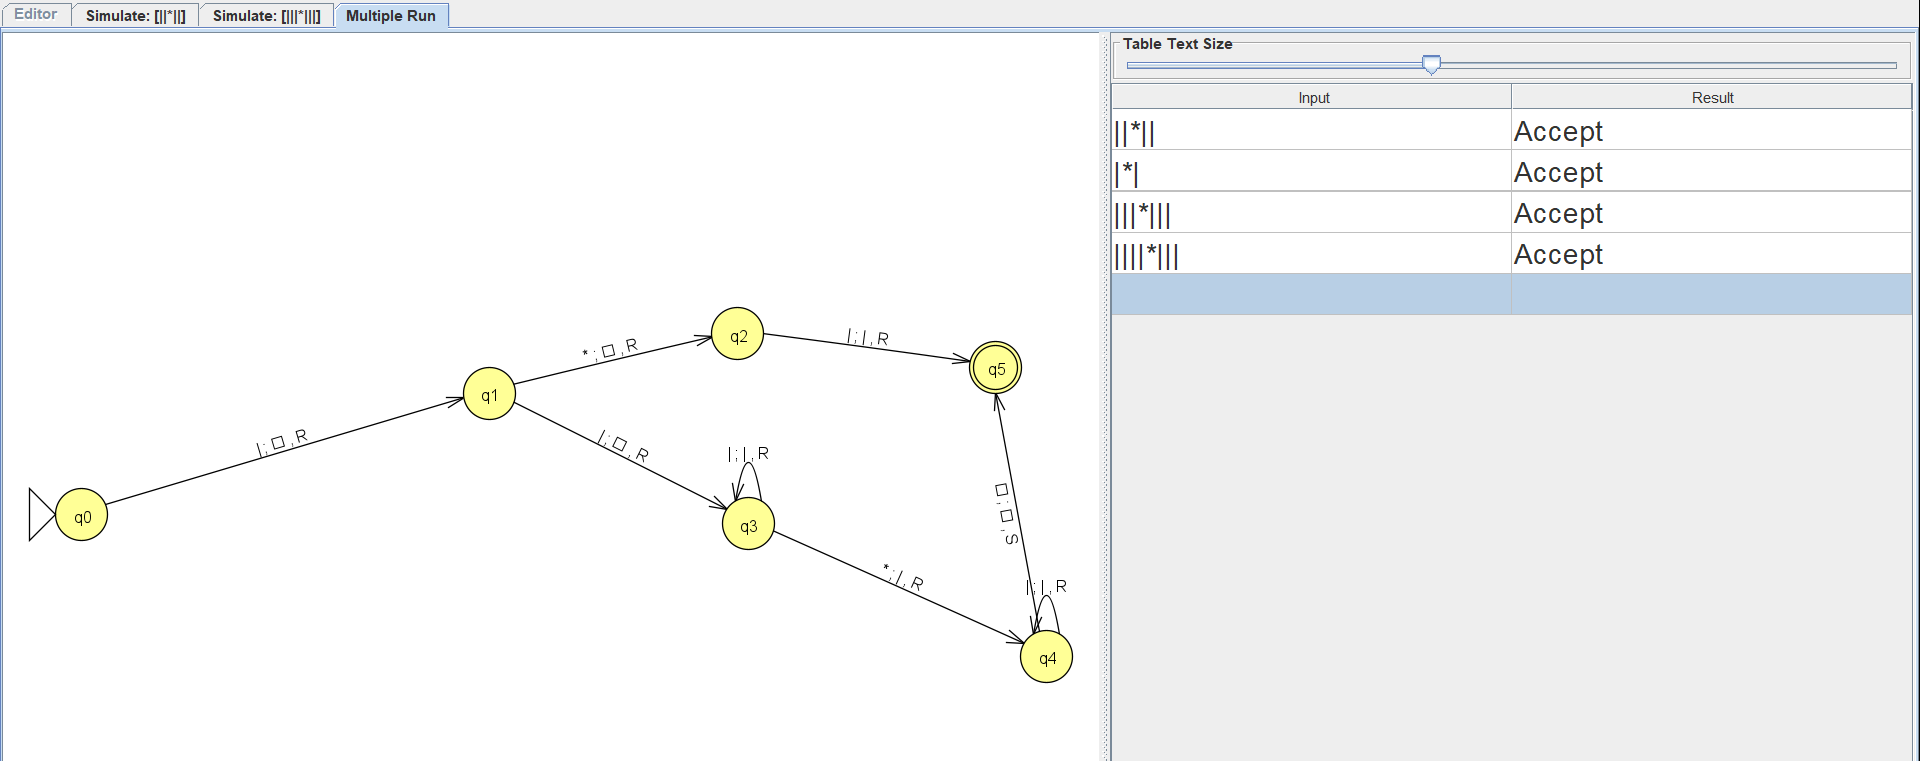
\includegraphics[scale=0.35]{TM.png}
  \item Define a recursive function for the sum of three values.
    \begin{center}
      $<$$<\pi^1_1|\sigma(\pi^3_3)>|\sigma(\pi^4_4)>$
    \end{center}
        
  \item Implement a WHILE program that computes the sum of three values. You
   must use an auxiliary variable that accumulates the result of the sum.\\
        $X4:=X1\\
        WHILE$ $X2 \not =  0$ $do\\
            X4:=X4+1\\
            X2:=X2-1\\
        od\\
        WHILE$ $X3 \not =  0$ $do\\
        X4:=X4+1\\
        X3:=X3-1\\
        od\\
        WHILE$ $X1 \not =  0$ $do\\
            X4:=X4+1\\
            X1:=X1-1\\
        od\\
        X1:=X4$

\end{enumerate}

\pagebreak



\end{document}